% 等体过程
% 等体过程|体积|压强|状态方程|做功

\pentry{理想气体状态方程\upref{PVnRT}}

等体过程的特征是气体的体积保持不变,即$V $为常量,$\mathrm dV=0$.设有一气缸,活塞保持固定不动,把气缸连续地与一系列有微小温度差的恒温热源相接触,使气体的温度逐渐上升,压强增大,但是气体的体积保待不变.这样的准静态过程是一个\textbf{等体过程(isochoric process)},如\autoref{EqVol_fig1}所示.
\begin{figure}[ht]
\centering
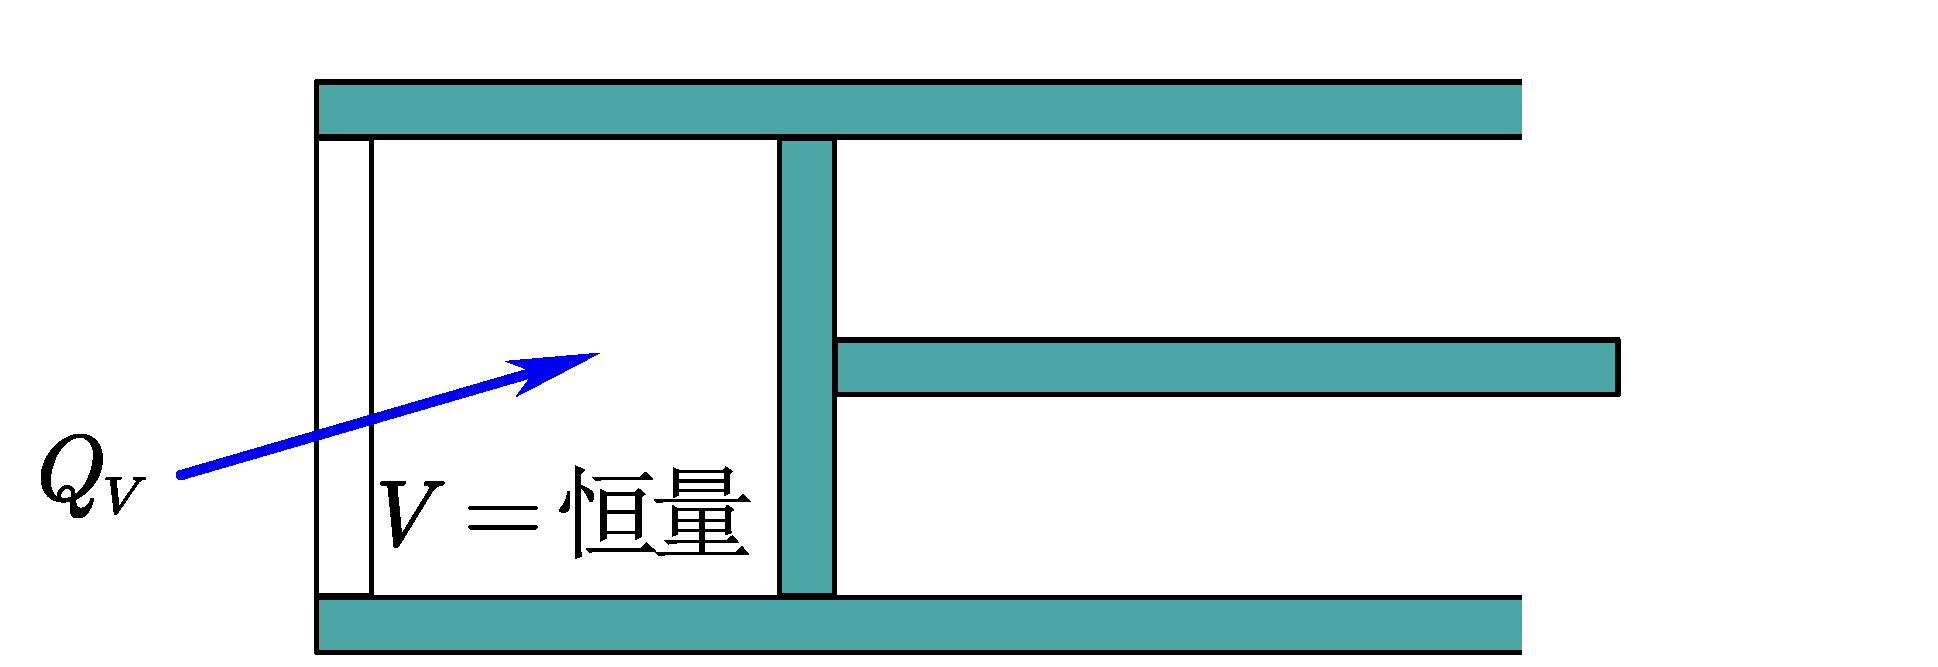
\includegraphics[width=10cm]{./figures/EqVol_1.pdf}
\caption{气体的等体过程} \label{EqVol_fig1}
\end{figure}
如\autoref{EqVol_fig2}所示,在等体过程中, $\mathrm dV=0$,所以$\delta W=0$.根据热力学第一定律,得
\begin{equation} \label{EqVol_eq1}
\delta Q_{V}=\mathrm{d} E 
\end{equation}
\begin{figure}[ht]
\centering
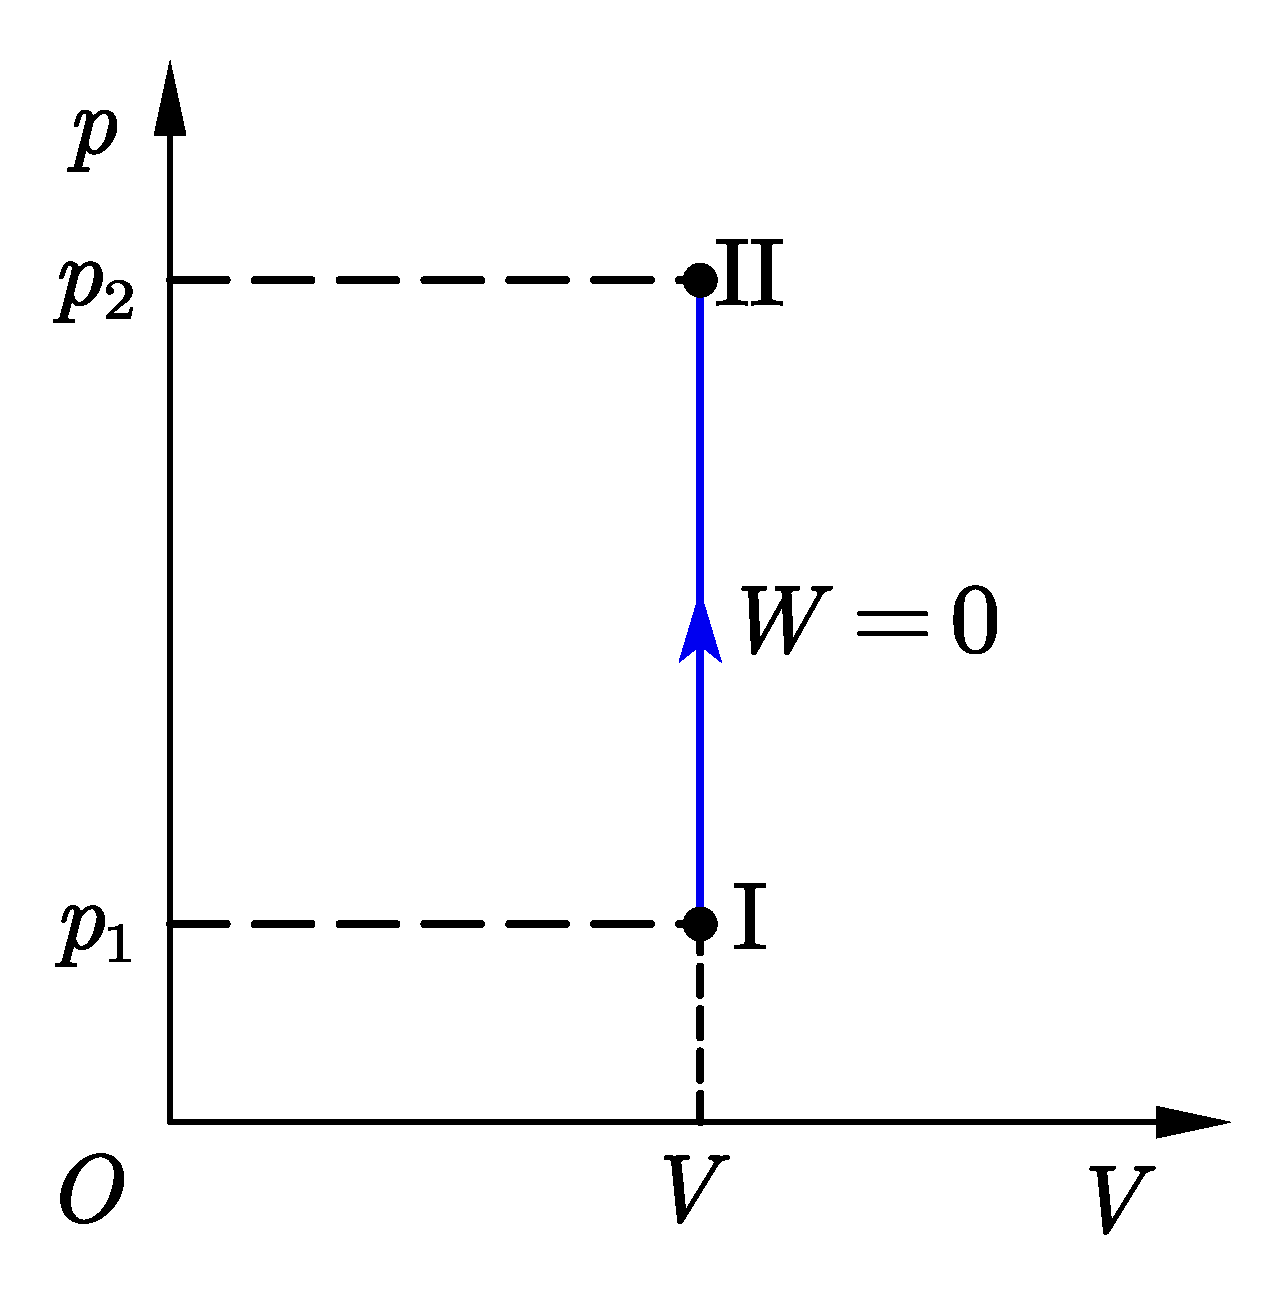
\includegraphics[width=5cm]{./figures/EqVol_2.pdf}
\caption{等体过程中功的计算} \label{EqVol_fig2}
\end{figure}
为了计算向气体传递的热量,我们要用到摩尔热容的概念:同一种气体在不同过程中,有不同的热容.最常用的是等体过程与等压过程中的两种热容.气体的\textbf{摩尔定容热容(molar heal capacity at constant volume)},是指$1 \rm mol$气体在体积不变的条件下,温度改变$1\mathrm{K}$(或$1^\circ \mathrm{C}$)所吸收或放出的热量,用$C_{V,m}$表示,其值可由实验测定.这样,质量为$m $的气体在等体过程中,温度改变$\mathrm dT $时所需要的热量就是
\begin{equation} \label{EqVol_eq2}
\delta Q_{V}=\frac{m}{M} C_{V, {m}} \mathrm{d} T
\end{equation}
作为$C_{V,m}$的定义式,可将上式改成写成:
\begin{equation} 
C_{V, m}=\frac{\delta Q_{V}}{\frac{m}{M} \mathrm{d} T}
\end{equation}
把\autoref{EqVol_eq2}代入\autoref{EqVol_eq1},即得:
\begin{equation} \label{EqVol_eq3}
\mathrm{d} E=\frac{m}{M} C_{V, m} \mathrm{d} T
\end{equation}

我们这里需要指出的一点是,\autoref{EqVol_eq3}是计算过程中理想气体内能变化的通用式子,不仅仅适用于等体过程.我们知道,理想气体的内能只与温度有关,所以一定质量的理想气体在不同的状态变化过程中,如果温度的增量$\mathrm dT $相同,那么气体所吸取的热量和所做的功虽然随过程的不同而异,但是气体内能的增量却相同,与所经历的过程无关.那么我们看,现在从等体过程中,我们得到了理想气体温度升高$\mathrm dT $时,内能的增量由\autoref{EqVol_eq3}给出,那么在任何过程中,都是可以用这个式子来计算理想气体的内能增量的.

我们知道,理想气体的内能为
\begin{equation}
E=\frac{m}{M} \frac{i}{2} R T
\end{equation}
由此得
\begin{equation} \label{EqVol_eq4}
\mathrm{d} E=\frac{m}{M} \frac{i}{2} R \mathrm{d} T
\end{equation}
把\autoref{EqVol_eq4}与\autoref{EqVol_eq3}相比较,我们可以看出:
\begin{equation}
C_{V, m}=\frac{i}{2} R
\end{equation}
上式说明,理想气体的摩尔定容热容是\textbf{一个只与分子的自由度有关的量,它与气体的温度无关}.对于单原子分子气体$i=3, C_{V, m}=12.5 \mathrm{J} /(\mathrm{mol} \cdot \mathrm{K})$;对于双原子分子气体,不考虑分子的振动,则$i=5, C_{V, {m}}=20.8 \mathrm{J} /(\mathrm{mol} \cdot \mathrm{K})$;对于多原子分子气体,不考虑分子的振动,则$i=6, C_{V, {m}}=24.9 \mathrm{J} /(\mathrm{mol} \cdot \mathrm{K})$.
